\documentclass{standalone}
\usepackage{tkz-euclide}

\begin{document}

\colorlet{input}{red!80!black}
\colorlet{output}{red!70!black}
\colorlet{triangle}{orange!40}

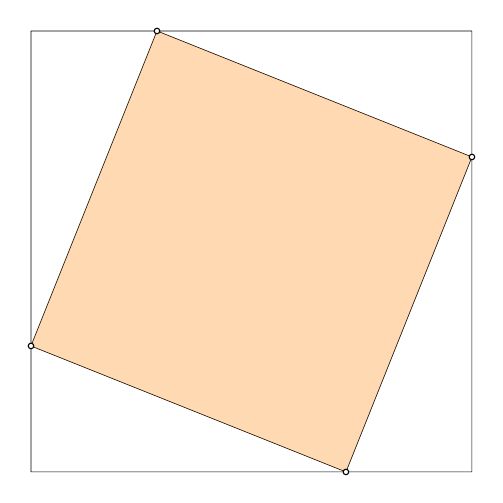
\begin{tikzpicture}[scale=.8]

\tkzDefPoint(0,0){A_1}
\tkzDefPoint(7,0){A_2}
\tkzDefPoint(7,7){A_3}
\tkzDefPoint(0,7){A_4}

 \foreach \an [count=\i] in {0,90,180,270}
 {\tkzDefShiftPoint[A_\i](\an:5){B_\i}
 \tkzDefShiftPoint[A_\i]({\an+90}:2){C_\i}
 \tkzDrawPolygon(A_\i,B_\i,C_\i)
 % \tkzLabelSegment[swap](A_\i,B_\i){$a$}
 % \tkzLabelSegment[swap](B_\i,C_\i){$c$}
 % \tkzLabelSegment[swap](C_\i,A_\i){$b$}
 % \tkzDrawPolygon[fill=blue,opacity=.3](A_\i,B_\i,C_\i)
 % \tkzDrawPoints[fill=white](A_\i)
 }
\tkzDrawPolygon[fill=orange,opacity=.3](B_1,B_...,B_4)
\tkzDrawPoints[fill=white,size=2](B_1,B_...,B_4)



\end{tikzpicture}



\end{document}
